% !TEX root = ../Thesis.tex
\acresetall
\myChapter{Discussion}\label{ch:discussion}
\begin{flushright}{\slshape And as soon as I'm done with these waffles, I shall discuss my evil  plan!} \\ \medskip
    --- \defcitealias{Zim}{Invader Zim}\citetalias{Zim} \citep{Zim}
\end{flushright}
\begin{flushright}{\slshape No discussion!} \\ \medskip
    --- Jean Reno as\defcitealias{Leon}{Léon}\citetalias{Leon} \citep{Leon}
\end{flushright}
\vspace{52mm}
The tomographic data obtained at the beamline for \ac{tomcat} offers an unmatched three-dimensional insight into the mammalian lung. Even if images of the terminal airway ends with higher resolution than the ones obtained at \ac{tomcat} have been obtained with scanning \ac{em}\todo{citation $\rightarrow$ Dani Studer?}, those images do not permit a full three-dimensional reconstruction of the terminal airway ends, they are only useful for understanding the surface structure of a sample. Using standard \ac{em} is impossible to visualize the larger three-dimensional structure of the terminal airway ends inside the lung since the sample has to be sectioned prior to acquiring images using this method, which essentially destroys the full three-dimensional information.

Tomography in contrast offers a non-destructive insight into the lung, tomographic microscopy using \ac{uct} enables the study of the major airways of swine~\cite{Litzlbauer2006}, rat~\cite{Langheinrich2004a,Sharif2010} or mice lung~\cite{Langheinrich2004,Ritman2005} and while \ac{srxtm} and \ac{wf-srxtm} enable the study of the functional lung units of the lung, the so-called acini with unmatched resolution and precision.

In this work three imaging methods based on ultrahigh resolution tomographic data of the terminal airway have been presented, the following sections discuss the major notable points of each of them.

\section{Multimodal Imaging}
The method presented in chapter~\ref{ch:xrm2008} combines the advantages of tomographic imaging and \ac{em} into a multimodal imaging approach for the analysis of inhaled particles in the lung. The tomographic data provides the unrestricted three-dimensional information on the location of sub-micron particles in the terminal airway tree which is combined with the extremely high resolution of the \ac{em}-images for the precise analysis of those particles in the lung tissue.

Exposure to ultra-fine particles and nanoparticles produces by environmental or industrial sources is an important health problem. It is expected that inhaled particles are deposited in specific locations in the lung\todo{citation $\rightarrow$ Christian Mühlfeld?}. With currently available methods, the exact location of these deposition sites in relation to the airways tree cannot easily be analyzed. 

Classic histological sections analyzed using light and electron microscopy allow for a precise location of the inhaled particles in relation to the tissue, \ie make it possible to analyze the interaction of the particles with alveolar macrophages and epithelial cells~\cite{Muhlfeld2008}. But the precise localization of these interaction sites inside the airway tree are impossible to extract using histological sections since the three-dimensional structure of the sample is destroyed.

Registration of classic histological slices with the three-dimensional data obtained through \ac{srxtm} make it possible to localize sites of interaction along the airway tree inside the three-dimensional structure of the terminal airways. The method presented in chapter~\ref{ch:xrm2008} was only little more than a proof of concept in terms of the registration between the two imaging modalities. Careful alignment of the sample prior to physical sectioning made registration straightforward, since the images only needed to be corrected for rotation and translation to be able correlate between a physical slice imaged using \ac{em} and a virtual slice of the \ac{srxtm} dataset.

Figure~\ref{fig:correlation} shows the three-dimensional situation of different alignment situations of the two multimodal datasets. The situation shown in figure~\ref{subfig:correlation-planar} can be achieved through careful alignment of the sample prior to histological sectioning and corresponds to the situation presented in chapter~\ref{ch:xrm2008}. The fully unrestricted three-dimensional information of the airway tree can be matched with highest resolution two-dimensional information about the particle location in or around the tissue in the lung\todo{what else can we discuss here? Skeletonization? Or is it enough to do this in the outlook?}.

Figures~\ref{subfig:correlation-arbitrary1} and \ref{subfig:correlation-arbitrary3} depict situations where the two datasets are arbitrarily orientated with one or multiple degrees of rotation, respectively.

\renewcommand{\imsize}{\linewidth}
\begin{figure}[h]
	\centering
	\pgfmathsetlength{\imagewidth}{\imsize}%
	\pgfmathsetlength{\imagescale}{\imagewidth/1586}%
	\def\x{1160}
	\def\y{364}% scalebar-y at 90% of height of y=404px
	\subfloat[Planar orientation of slice]{%
		\begin{tikzpicture}[x=\imagescale,y=-\imagescale]
			\node[anchor=north west,inner sep=0pt,outer sep=0pt] at (0,0) {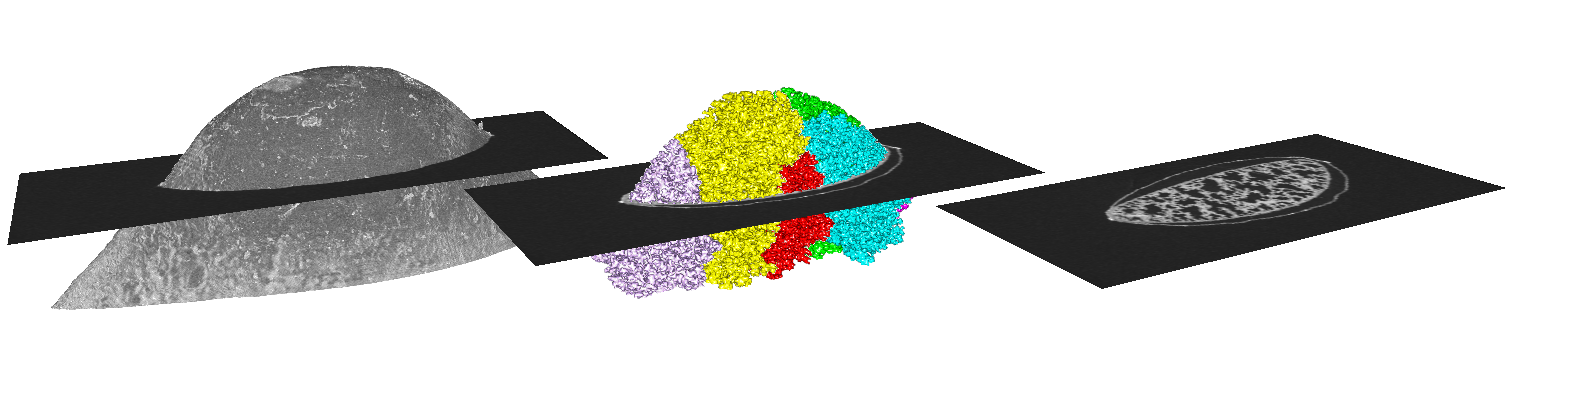
\includegraphics[width=\imagewidth]{img/discussion/R108C21Bt-mrg-planar}};
			% 515px = 4.3423mm > 100px = 844um > 59px = 500um, 12px = 100um
			%\draw[orange,|-|,thick] (537,266) -- (1043,172) node [sloped,midway,above] {\SI{4.3423}{\milli\meter} (2934px)};
			\draw[|-|,thick] (\x,\y) -- (\x+118,\y) node [right] {\SI{1}{\milli\meter}};
		\end{tikzpicture}%
		\label{subfig:correlation-planar}
		}\\%
	\subfloat[Arbitrary orientation of slice, one degree of freedom]{%
		\begin{tikzpicture}[x=\imagescale,y=-\imagescale]
			\node[anchor=north west,inner sep=0pt,outer sep=0pt] at (0,0) {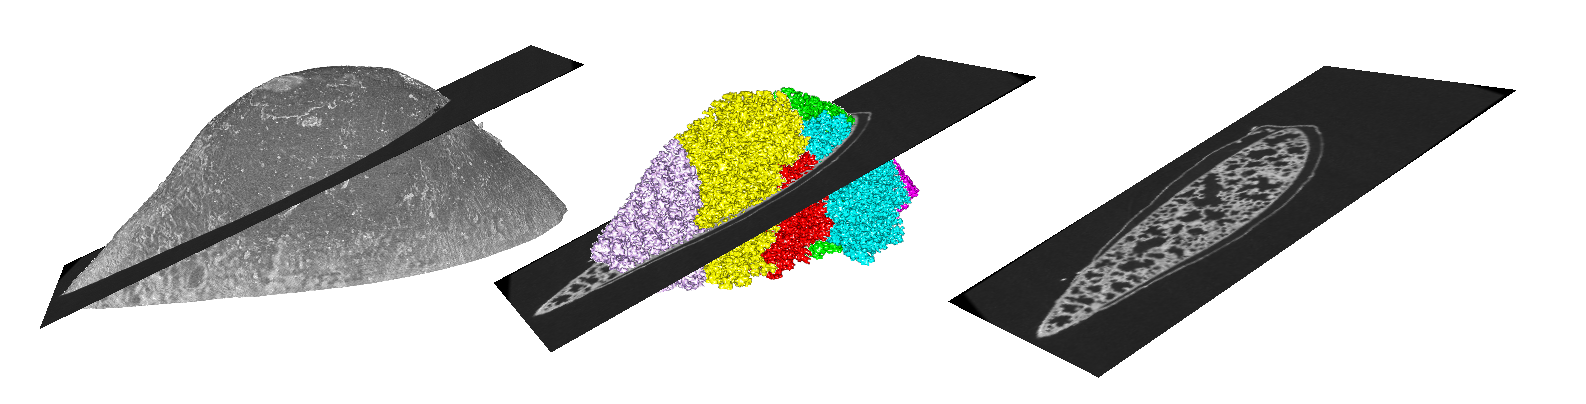
\includegraphics[width=\imagewidth]{img/discussion/R108C21Bt-mrg-arbitrary1}};
			% 515px = 4.3423mm > 100px = 844um > 59px = 500um, 12px = 100um
			%\draw[white,|-|,thick] (537,266) -- (1043,172) node [sloped,midway,above] {\SI{4.3423}{\milli\meter} (2934px)};
			\draw[|-|,thick] (\x,\y) -- (\x+118,\y) node [right] {\SI{1}{\milli\meter}};
		\end{tikzpicture}%
		\label{subfig:correlation-arbitrary1}
		}\\%
	\subfloat[Arbitrary orientation of slice, multiple degrees of freedom]{%
		\begin{tikzpicture}[x=\imagescale,y=-\imagescale]
			\node[anchor=north west,inner sep=0pt,outer sep=0pt] at (0,0) {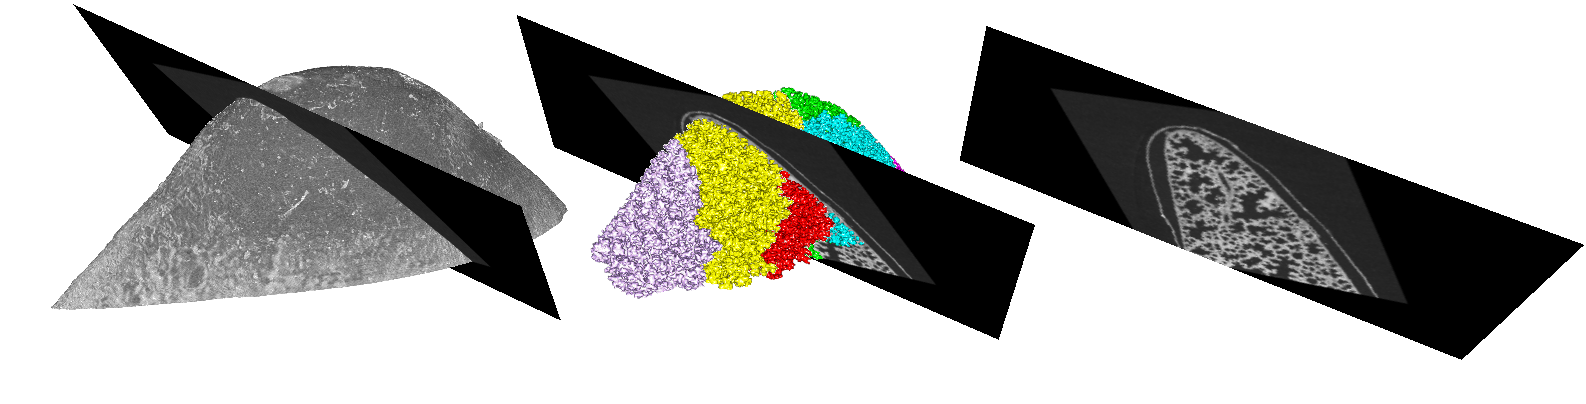
\includegraphics[width=\imagewidth]{img/discussion/R108C21Bt-mrg-arbitrary3}};
			% 515px = 4.3423mm > 100px = 844um > 59px = 500um, 12px = 100um
			%\draw[white,|-|,thick] (537,266) -- (1043,172) node [sloped,midway,above] {\SI{4.3423}{\milli\meter} (2934px)};
			\draw[|-|,thick] (\x,\y) -- (\x+118,\y) node [right] {\SI{1}{\milli\meter}};
		\end{tikzpicture}%
		\label{subfig:correlation-arbitrary3}
		}%
	\caption[Multimodal Imaging]{Multimodal Imaging: Alignment of datasets from two imaging modalities. Left: Sample from \ac{srxtm} with overlayed \ac{em} image (gray-scale inverted, thus dark slice). Center: Five independent airway segments have been extracted and are three-dimensionally visualized with overlayed \ac{em}-image. Right: \ac{em}-image shown with three-dimensional orientation in relation to the \ac{srxtm} dataset. \subref{subfig:correlation-planar}: Planar orientation of the slice obtained with the second imaging modality. Through careful orientation of the sample prior to sectioning a registration is straightforward, since only the rotation in the plane of the slice and the different magnification have to be taken into account. \subref{subfig:correlation-arbitrary3}: Pitch-angle~\cite{YawPitchRoll} rotation between the two datasets. \subref{subfig:correlation-arbitrary3}: Pitch and roll rotation between the two datasets.}
	\label{fig:correlation}
	\todo[inline]{Slice is not multimodal but from \ac{srxtm}-set, so essentially I'm lying\dots $\rightarrow$ Do we need to show a LM or EM-slice or is this enough for concept?}
\end{figure}

Current work in our group focuses on an automatic registration method taking into account all six degrees of freedom \ie rotation and translation in the x, y and z-plane. First results have already been presented as a master thesis by Sébastien \citet{Barre2009}.

\section{Finite Element}
The results presented in chapter~\ref{ch:tsuda2008} focus more on the structural analysis of the gas-exchange region of the lung. The alveolar structure of the pulmonary acinus plays a vital role in gas exchange function. Using an analytical method which mapped a \ac{fe} representation of the terminal airways over a three-dimensional reconstruction of a \ac{srxtm} dataset we accurately reconstructed the gas exchange regions of the lung in three dimensions with ultrahigh resolution of \SI{1.48}{\micro\meter} per voxel.

To our knowledge it has never before been possible to three-dimensionally analyze the structure-function relationship of the parenchymal region of the lung in such detail. \citet{Berend1991} performed an analysis of the peripheral region of one human lung using serial sections studied by light microscopy. They were able to analyze the structure of one partical acinus through formidable effort and stated that the process proved to be very difficult and time consuming. \citet{Litzlbauer2006} analyzed porcine lungs using \ac{uct} but suggest to favor \ac{srxtm} over \ac{uct} to enhance the quality of morphometric analysis of the terminal airway structure.

Using \ac{srxtm} it has been not only been possible to visualize the alveolar region of rat lung samples, but also to assess and match morphological parameters of the computed three-dimensional reconstruction to prior stereologically assessed parameters of these lungs.

Since the reconstructed datasets have been directly elementarized using a \ac{fe} mesh lung tissue and air space were not only three-dimensionally visualized, but also immediately prepared for further analysis of the terminal airway region. Different morphological parameters were assessed and the \ac{fe} meshing prepared the resulting dataset for subsequent \ac{cfd} analysis of the airflow in the lung~\todo{moar?}.

\section{Widefield SRXTM}
\begin{itemize}
	\item tomography in general
	\item widefieldscan application
	\item skeletonization
	\item acinus detection \threed, marking in \twod makes it ``more understandable'' than on classic slices, see outlook in chapter~\ref{ch:outlook} and figure~\ref{fig:acinus overlay}.
\end{itemize}